\documentclass{beamer}
\usetheme[
          titleline=true,% Show a line below the frame title.
          titlepagelogo=ucmlogo,% Logo for the first page.
          logowidth=0.3,
          authorwidth=0.5,
          pageofpages = de
          ]{Zaragoza}

\author{Jorge Alda Gallo}
\title{Nuevas aplicaciones del modelo de Coleman-Weinberg}
\institute{Departamento de Física Teórica I, Universidad Complutense de Madrid}
\date{4 de Julio de 2016}
\logo{
\includegraphics[height=30px]{ucmlogo}}
\usecolortheme{ucm}
\usepackage[utf8]{inputenc}

<<<<<<< HEAD
\usepackage{siunitx}

\newcommand{\dif}{\mathrm{d}}
\newcommand{\expo}[1]{\mathrm{e}^{#1}}
\newcommand{\tr}{\mathrm{tr}}
\newcommand{\sla}[1]{\!\not\!#1\,}

=======
>>>>>>> 767691b7810acbd7db856a1b2bebff0280909acc
\setbeamertemplate{section in toc}[sections numbered]
\setbeamertemplate{subsection in toc}[sections numbered]
\usefonttheme[onlymath]{serif}

\begin{document}
\begin{frame}[t, plain]
\titlepage
\end{frame}

\begin{frame}[t]{Índice}
\tableofcontents
\end{frame}

\section{Introducción}
<<<<<<< HEAD
\begin{frame}{Introducción}
\begin{itemize}
\item Generalización del modelo de Coleman-Weinberg para describir el origen de la masa del bosón de Higgs.
\item Nuevo multiplete escalar en un grupo $\mathsf{SU}(N_S)$.
\item La masa del escalar está condicionada por la renormalizabilidad de la teoría y la unificación de las constantes. 
\item El escalar se acola al resto del modelo estándar, lo que determina su producción en aceleradores de partículas y su desintegración.
\end{itemize}
\end{frame}
\subsection{El modelo electrodébil y el mecanismo de Higgs}
\begin{frame}{El modelo electrodébil y el mecanismo de Higgs}
\begin{itemize}
%\item<1> El mecanismo de Higgs explica las masas de los bosones $W$ y $Z$ y de los fermiones quirales.
\item<only@1> El campo de Higgs es un doblete escalar de $\mathsf{SU}(2)_L \times \mathsf{U}(1)_Y$ con un potencial
\begin{equation}\label{eq:HiggsPotential}
\qquad V = m^2 H^\dagger H + \lambda_h (H^\dagger H)^2\ ; \qquad\qquad m^2<0\ .
\end{equation}
\item<only@1> El campo de Higgs tiene un mínimo que rompe la simetría electrodébil con $v_h = \sqrt{2}\langle H\rangle =\SI{246.2}{\giga\electronvolt}$, donde 
\begin{equation}
m^2 = -2\lambda_h v_h^2\ .
\end{equation}
\item<only@1> La masa del bosón de Higgs está dada por la segunda derivada del potencial en el mínimo, 
\begin{equation}
m_h^2 = 2 \lambda_h v_h^2=-m^2\ .
\end{equation}
\item<only@1> Las excitaciones respecto al mínimo se parametrizan como
\begin{equation}
H(x) =\frac{1}{\sqrt{2}} \begin{pmatrix}0 \\ h(x) +  v_h\end{pmatrix}\ . \label{eq:HiggsExpansion}
\end{equation}

\item<only@2> El término cinético para el campo de Higgs es
{\scriptsize\begin{equation}
\mathcal{L}_{\mathrm{kin} H} = D_\mu H^\dagger D^\mu H\ , \qquad\qquad
D_\mu H = \left(\partial_\mu  - \frac{i}{2} g_1 B_\mu -i g_2 W_\mu^a \tau^a  \right) H\ .
\end{equation}}
\item<only@2> Una combinación de $W^3$ y $B$ es el fotón, el generador del subgrupo $\mathsf{U}(1)_{em}$ que no rompe el mecanismo de Higgs
\begin{equation}
A_\mu = \frac{g_1 W_\mu^3 + g_2 B_\mu }{\sqrt{g_1^2 + g_2^2}}\ ,\qquad\qquad
Z_\mu = \frac{g_2 W_\mu^3 - g_1 B_\mu }{\sqrt{g_1^2 + g_2^2}}\ .
\end{equation}
\item<only@2> Tras la ruptura electrodébil, el término cinético resulta
\begin{equation}
\mathcal{L}_{\mathrm{kin}H} = \frac{1}{2}(\partial_\mu h)^2 + \frac{g_2^2}{4} W_\mu^+ W^{\mu-} (v_h + h)^2 + \frac{g_1^2 + g_2^2}{8}Z_\mu Z^\mu (v_h + h)^2\ , \label{eq:WZmassterm}
\end{equation}
con lo que los bosones $W$ y $Z$ adquieren masa
\begin{equation}
m_W= \frac{g_2}{2} v_h \qquad\qquad m_Z = \frac{\sqrt{g_1^2 + g_2^2}}{2}v_h\ .
\end{equation}
\item<only@3> La masa de los fermiones proviene de interacciones de tipo Yukawa compatibles con las diferentes simetrías electrodébiles levógiros y dextrógiros
\begin{equation}
\mathcal{L}_e = - y_e \left[ \begin{pmatrix}\bar{\nu}_e & \bar{e} \end{pmatrix}_L H e_R + \bar{e}_R H^\dagger \begin{pmatrix}\nu_e\\ e\end{pmatrix}_L \right]\ . \label{eq:yukawae}
\end{equation} 
\item<only@3> Tras la ruptura electrodébil
\begin{equation}
\mathcal{L}_e = -\frac{v_h y_e}{\sqrt{2}} (\bar{e}_L e_R + \bar{e}_R e_L)- \frac{y_e}{\sqrt{2}} h (\bar{e}_L e_R + \bar{e}_R e_L) \ ,
\end{equation}
con lo cual la masa del fermión es
\begin{equation}
m_e = \frac{v_h y_e}{\sqrt{2}}\ .
\end{equation}
\end{itemize}
\end{frame}

\subsection{Problemas del mecanismo de Higgs}
\begin{frame}[t]{Problemas: estabilidad del vacío}
\begin{itemize}
\item El potencial del bosón de Higgs cambia con la escala debido a las correcciones cuánticas.
\item Debido al valor de $y_t$, el parámetro $\lambda_h$ podría hacerse negativo a altas energías.
\item El vacío electrodébil sería \textbf{metaestable}.
\end{itemize}
\begin{center}
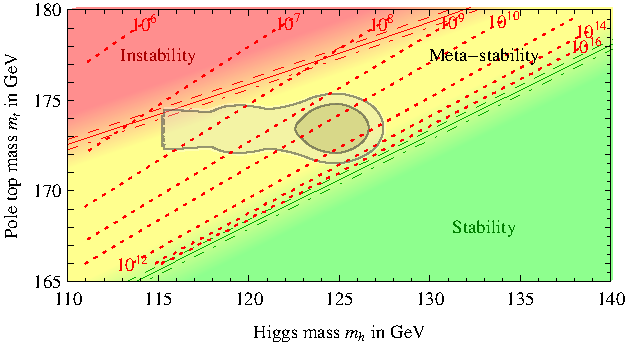
\includegraphics[width=0.7\textwidth]{stability}
{\scriptsize Fuente: arXiv:1112.3022}
\end{center}

\end{frame}

\begin{frame}{Problemas: jerarquía}
\begin{itemize}
\item $m$ es el único parámetro con dimensiones del modelo estándar.
\item Toda teoría de campos cuántica relativista incluye otra escala de energía, la escala de Planck $M_P$.
\item Por argumentos de naturalidad, $m$ y $M_P$ \textit{deberían} ser similares.
\item Sin embargo, $M_P$ es \textbf{17 órdenes de magnitud} mayor que $m$.  
\end{itemize}
\end{frame}

\subsection{El mecanismo de Coleman-Weinberg}
\begin{frame}{El mecanismo de Coleman-Weinberg}
\only<1>{
\begin{itemize}

\item Coleman y Weinberg (CW) propusieron un modelo con $m=0$.
\item La masa del bosón se debe a las correcciones radiativas al término cuártico (transmutación dimensional).
\item El potencial clásico es invariante de escala, y por lo tanto, libre del problema de la jerarquía.
\item La jerarquía entre la masa del Higgs y la escala de Planck está controlada exponencialmente por la evolución de $\lambda_h$ según el grupo de renormalización.
\end{itemize}}
\only<2>{
\begin{center}
\begin{figure}
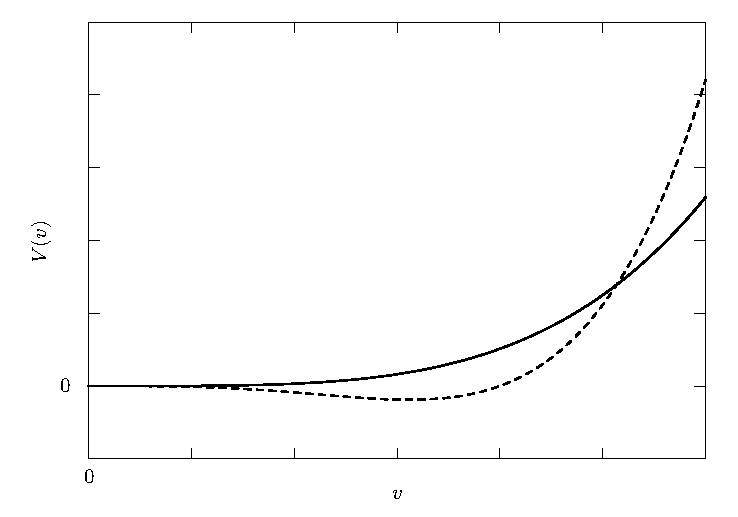
\includegraphics[width=0.8\textwidth]{../memoria/potential}
\end{figure}
\end{center}
}
\only<3>{
\begin{itemize}
\item Pero el modelo de C-W no predice la masa correcta del Higgs.
\item Si los fermiones no tuvieran masa, $m_h = \SI{10}{\giga\electronvolt}$. 
\item A medida que aumenta la masa de los fermiones disminuye $m_h$.
\item Si $m_t \geq m_W$, la masa del Higgs es negativa: el potencial tiene un máximo, y la simetría electrodébil no se rompe.
\end{itemize}
}
=======
\begin{frame}[t]{Introducción}

\end{frame}
\subsection{El modelo electrodébil y el mecanismo de Higgs}
\begin{frame}[t]{El modelo electrodébil y el mecanismo de Higgs}

\end{frame}

\subsection{Problemas del mecanismo de Higgs}
\begin{frame}[t]{Problemas del mecanismo de Higgs}

\end{frame}

\subsection{El mecanismo de Coleman-Weinberg}
\begin{frame}[t]{El mecanismo de Coleman-Weinberg}
>>>>>>> 767691b7810acbd7db856a1b2bebff0280909acc

\end{frame}

\section{El modelo}
<<<<<<< HEAD
\begin{frame}{El modelo}
\begin{itemize}
\item<only@1> El campo de Higgs $H$ sigue siendo un campo escalar sin masa en la representación fundamental de $\mathsf{SU}(2)_L\times \mathsf{U}(1)_Y$.
\item<only@1> Añadimos un campo escalar sin masa $S$ en la representación fundamental de $\mathsf{SU}(N_S)$.
\item<only@1> El potencial para los dos campos es
\begin{equation}\label{eq:CWpotential}
V = \lambda_h (H^\dagger H)^2 + \lambda_{hs} (H^\dagger H) (S^\dagger S) + \lambda_s (S^\dagger S)^2\ .
\end{equation}
\item<only@1> Las constantes de acoplamiento $\lambda_h$, $\lambda_s$ y $\lambda_{hs}$ son adimensionales.

\item<only@2> En primer lugar se rompe la simetría $\mathsf{SU}(N_S)$.
\item<only@2> El campo $S$ adquiere un vev $|S| = v_s + \frac{\sigma}{\sqrt{2}}$.
\item<only@2> La dependencia de las constantes de acoplamiento con la escala de energía se puede aproximar como $\lambda(|S|) = \beta \log(|S|/M)$:
\begin{subequations}
\begin{align}
\lambda_h\left(v_s + \frac{\sigma}{\sqrt{2}}\right) &\approx \lambda_h(v_s) + \beta_h \left(\frac{\sigma}{\sqrt{2}v_s}-\frac{\sigma^2}{4 v_s^2}\right)\ ,\\
\lambda_s\left(v_s + \frac{\sigma}{\sqrt{2}}\right) &\approx \lambda_s(v_s) + \beta_h \left(\frac{\sigma}{\sqrt{2}v_s}-\frac{\sigma^2}{4 v_s^2}\right)\ ,\\
\lambda_{hs}\left(v_s + \frac{\sigma}{\sqrt{2}}\right) &\approx \lambda_{hs}(v_s) + \beta_{hs} \left(\frac{\sigma}{\sqrt{2}v_s}-\frac{\sigma^2}{4 v_s^2}\right)\ .
\end{align}
\end{subequations}
\item<only@3> La condición para el mínimo de potencial es
\begin{equation}
\frac{\dif V_\mathrm{eff}}{\dif \sigma}\Big|_{\substack{\sigma=0\\ H=0}} = \frac{v_s^3}{\sqrt{2}}(4\lambda_s + \beta_s) = 0\ ,  \qquad 4\lambda_s = - \beta_s \ . \label{eq:minimum}
\end{equation}
\item<only@3> La masa del escalar $S$ es 
\begin{equation}
m_s^2 = \frac{\dif^2 V_\mathrm{eff}}{\dif \sigma^2}\Big|_{\substack{\sigma=0\\ H=0}} \! =\frac{v_s^2}{2} (12 \lambda_s +7\beta_s) =2\beta_s v_s^2 = -8 \lambda_s v_s^2\ .
\end{equation}
\item<only@4> El potencial se puede reescribir como
\begin{equation}
V_\mathrm{eff} = V_H (H) + V_S (\sigma) + V_\mathrm{int}(H, \sigma)\ ,
\end{equation}
\begin{subequations}
\begin{align}
V_H =& m^2 H^\dagger H + \lambda_h (H^\dagger H)^2\label{eq:quadraticCW}\ , \\
V_S =& \frac{m_s^2}{2} \sigma^2 + \sqrt{2}(\lambda_s \!\!+\!\!\beta_s)v_s \sigma^3 + \frac{\lambda_s \!\!+\!\!\beta_s}{4}\sigma^4 - \frac{\beta_s}{2^{5/2} v_s}\sigma^5 - \frac{\beta_s}{16 v_s^2}\sigma^6\  \label{eq:Spotential},\\
V_\mathrm{int} =& \frac{(2\lambda_{hs} + \beta_{hs})v_s}{\sqrt{2}}\sigma H^\dagger H + \frac{2\lambda_{hs} + 3\beta_{hs}}{4}\sigma^2 H^\dagger H\nonumber\\ &+ \frac{\beta_h}{\sqrt{2} v_s}\sigma (H^\dagger H)^2 - \frac{\beta_{hs}}{8 v_s^2}\sigma^4 H^\dagger H- \frac{\beta_h}{4 v_s^2}\sigma^2 (H^\dagger H)^2\ . \label{eq:interlagr}
\end{align}
\end{subequations}
\item<only@5> Aparece de manera automática un término de masa para $H$:
\begin{equation}
m^2 = -m_\eta^2 = 2 \lambda_{hs} v_s^2\ .
\end{equation}
\item<only@5> La masa del Higgs ya no es un parámetro libre.
\item<only@5> La ruptura espontánea de la simetría electrodébil procede de la manera habitual. Representaremos las excitaciones de $H$ respecto del vacío $v_h$ por el campo $\eta$.	 

\end{itemize}
\end{frame}

\section{Grupo de Renormalización}
\begin{frame}{Grupo de Renormalización}
\only<1-3,5-6>{
\begin{itemize}
\item<only@1> Ecuaciones del grupo de renormalización a 1 loop:
\begin{align}
16\pi^2 \frac{\dif \lambda_h}{\dif (\ln \mu)} =& 24\lambda_h^2 + N_S \lambda_{hs}^2-6 y_t^4 +12y_t^2 \lambda_h \ ,\\
16\pi^2 \frac{\dif \lambda_s}{\dif (\ln \mu)} =& 4(4+N_S)\lambda_s^2 + 2\lambda_{hs}^2 - 6 \frac{N_S^2-1}{N_S}g_4^2 \lambda_s \nonumber \\ &+ \frac{3}{4} \frac{N_S^3 + N_S^2-4N_S+2}{N_S^2}g_4^4 \ , \\
16\pi^2 \frac{\dif \lambda_{hs}}{\dif (\ln \mu)} =& \lambda_{hs} \Big[ 4\lambda_{hs} +12\lambda_h +(4N_S+4)\lambda_s \nonumber \\ &-3 \frac{N_S^2-1}{N_S}g_4^2 +6y_t^2\Big]\ ,
\end{align}
\item<only@2> La condición de mínimo $4\lambda_s=-\beta_s$, cuando $g_4=0$, es
\begin{equation}\label{eq:lhs}
\lambda_{hs}=-\sqrt{-32\pi^2 \lambda_s -2(4+N_S)\lambda_s^2}\ .
\end{equation}
\begin{equation}
|\lambda_s| \leq \frac{16\pi^2}{4+N_S}\ . \label{eq:lim_ls}
\end{equation}
\begin{equation}\label{eq:ls}
\lambda_s = \frac{-16\pi^2}{4+N_S+\frac{8m_\eta^4}{m_\sigma^4}}\ .
\end{equation}
\item<only@3> \textbf{Escenario 1:} $|\lambda_s|\to 0$
\begin{itemize}
\item La condición de mínimo es
\begin{equation}
\lambda_{hs} = -\sqrt{32\pi^2 \lambda_s}\ ,
\end{equation}
\begin{equation}
m_\sigma = 2 m_\eta \left(\frac{\lambda_s}{32\pi^2}\right)^{1/4}\ .
\end{equation}
\item Para que el modelo sea perturbativo ($|\lambda| \leq 3$) a bajas energías, $m_\sigma \leq \num{0.17}m_\eta$.
\item El valor de $N_S$ no afecta.
\end{itemize}
\item<only@5> Las constantes de acoplamiento crecen con la escala de energía.
\item<only@5> Se alcanza un polo de Landau a energías relativamente bajas...
\item<only@5> ...a no ser que $m_\sigma$ sea muy pequeño.

\item<only@6> \textbf{Escenario 2:}
\begin{equation}
|\lambda_s| = \frac{16\pi^2}{4+N_S} - \delta \ \ \mathrm{as}\ \ \delta\to 0^+\ ,
\end{equation}
 \begin{itemize}
\item La condición de mínimo es 
\begin{equation}
\lambda_{hs} = -\sqrt{32\pi^2 \delta}\ ,
\end{equation}
\begin{equation}
m_\sigma = 2 m_\eta \frac{1}{\sqrt{N_S + 4 }}\left(\frac{8\pi^2}{\delta}\right)^{1/4}\ .
\end{equation}
\item Para que sea perturbativo a bajas energías, $N_S \geq 50$.
\item No hay restricciones sobre $m_\sigma$.
\end{itemize}
\end{itemize}
}


\begin{center}
\includegraphics<4>[width=0.7\textwidth]{../memoria/scenario2}
\only<4>{\\$m_\sigma = \SI{10}{\giga\electronvolt}\qquad\qquad N_S=2\ .$}
\includegraphics<7>[width=0.7\textwidth]{../memoria/scenario1}
\only<7>{\\$m_\sigma = \SI{3}{\tera\electronvolt}\qquad\qquad N_S=100\ .$}
\end{center}
\end{frame}

\section{Mezcla de los escalares}
\begin{frame}{Mezcla de los escalares}
\only<1,3>{
\begin{itemize}
\item<only@1> Los campos $\sigma$ y $\eta$ son ambos escalares 
\item<only@1> El potencial de interacción contiene términos proporcionales a $\sigma\eta$.
\item<only@1> Por lo tanto, $\sigma$ y $\eta$ no son autoestados de masa, sino que se mezclarán.
\item<only@1> Los autoestados de masa se obtienen diagonalizando los términos cuadráticos del potencial.
\begin{equation}
h = \eta \cos \theta - \sigma \sin \theta \qquad\qquad s = \eta \sin \theta + \sigma \cos \theta\ ,
\end{equation}

\begin{equation}
\theta = \frac{1}{2} \tan^{-1} \frac{2m_{\eta\sigma}^2}{m_\sigma^2 - m_\eta^2}\ .
\end{equation}
\item<only@1> $\theta$ es el ángulo de mezcla escalar.

\item<only@3> En el escenario 1, el término cuadrático no es definido positivo, y el potencial no tiene un mínimo.
\item<only@3> Para que el potencial sea definido positivo, $m_\sigma \geq m_\eta$.
\item<only@3> En el escenario 2, el ángulo de mezcla es despreciable: $\eta \approx h$ es el bosón de Higgs y $\sigma \approx s$ es el nuevo escalar.
\item<only@3> Las masas de los autoestados de masa son
\begin{align}
m_h^2 = m_\eta^2 \cos^2 \theta + m_\sigma^2 \sin^2 \theta - 2 m_{\eta\sigma}^2 \sin \theta \cos \theta\ , \\
m_s^2 = m_\sigma^2 \cos^2 \theta + m_\eta^2 \sin^2 \theta + 2 m_{\eta\sigma}^2 \sin \theta \cos \theta\ .
\end{align}
\end{itemize}}

\begin{center}
\includegraphics<2>[width=0.8\textwidth]{../memoria/angle}
\end{center}

\end{frame}


\section{Unificación de las constantes}
\begin{frame}{Unificación de las constantes}
\only<1,4>{
\begin{itemize}
\item<only@1> En el escenario 2, se ha visto que las tres constantes tienden a un valor común a altas energías.
\item<only@1> Muchas teorías más allá del modelo estándar proponen una unificación de las constantes de acoplamiento (GUT).
\item<only@1> Definimos una medida para la unificación de las tres constantes
\begin{equation}
d = \frac{1}{3}(|\lambda_h - \lambda_s| + |\lambda_h - \lambda_{hs}|+ |\lambda_s - \lambda_{hs}|)\ ,
\end{equation}
\item<only@1> y la empleamos para determinar la escala de energía $\mu_U$ en la que se produce la unificación.

\item<only@4> El factor determinante para la unificación es $m_\sigma$, mientras que $N_S$ solo produce pequeñas modificaciones. Un valor elevado de $N_S$ disminuye la distancia de unificación, 
\item<only@4> Si $m_\sigma \leq \SI{400}{\giga\electronvolt}$, no hay unificación antes de la escala de Planck.
\item<only@4> Para conseguir una escala de unificación cercana a la escala GUT (\SI{e16}{\giga\electronvolt}), se necesita $m_\sigma \approx \SI{4}{\tera\electronvolt}-\SI{8}{\tera\electronvolt}$. 
\end{itemize}
}
\begin{center}
\includegraphics<2>[width=0.8\textwidth]{../memoria/GUTdistance}
\includegraphics<3>[width=0.8\textwidth]{../memoria/GUTscale}
\end{center}
\end{frame}

\section{Fenomenología}
\begin{frame}{Fenomenología}
\only<1>{
\begin{itemize}
\item $S$ es un multiplete de $N_S$ partículas escalares inicialmente sin masa que solamente interaccionan con el campo de Higgs.
\item Uno de los escalares, $s$, adquiere masa y se mezcla con el bosón de Higgs.
\item Por motivo de esta mezcla, $s$ interacciona con el resto del modelo estándar en los mimsos canales que el bosón de Higgs, pero con la amplitud suprimida un factor $\sin \theta$.
\item Posibilidad de confrontar el modelo con resultados experimentales.
\end{itemize}}
\begin{center}
\includegraphics<2>[width=0.95\textwidth]{../memoria/diagrams}
\end{center}
=======
\begin{frame}[t]{El modelo}

\end{frame}

\section{Grupo de Renormalización}
\begin{frame}[t]{Grupo de Renormalización}

\end{frame}

\section{Mezcla de los escalares}
\begin{frame}[t]{Mezcla de los escalares}

\end{frame}

\section{Unificación de las constantes}
\begin{frame}[t]{Unificación de las constantes}

\end{frame}

\section{Fenomenología}
\begin{frame}[t]{Fenomenología}

>>>>>>> 767691b7810acbd7db856a1b2bebff0280909acc
\end{frame}

\subsection{Desintegraciones}
\begin{frame}[t]{Desintegraciones}
<<<<<<< HEAD
\only<1-3>{
\begin{itemize}
\item<only@1> Canal de desintegración $s\to hh$.
\begin{itemize}
\item Término en el lagrangiano $
\mathcal{L}_{hhs} = \frac{\kappa}{2} h^2 s\ $
{\scriptsize \begin{align}
\kappa =& \left(\frac{(2\lambda_{hs} + \beta_{hs})v_s}{\sqrt{2}} + 6 v_h^2\frac{\beta_h}{\sqrt{2} v_s} \right)\cos^3 \theta \nonumber\\
&+ \left(-4\sqrt{2}v_h \frac{2\lambda_{hs} + 3\beta_{hs}}{4} - 8\sqrt{2}v_h^3  \frac{\beta_h}{4 v_s^2} \right)\cos^2\theta \sin \theta \\
&+ \left(-2\frac{(2\lambda_{hs} + \beta_{hs})v_s}{\sqrt{2}} -12 v_h^2\frac{\beta_h}{\sqrt{2} v_s} +6\sqrt{2}(\lambda_s+\beta_s) v_s \right)\cos\theta \sin^2\theta \nonumber\\
&+\left(2\sqrt{2}v_h \frac{2\lambda_{hs} + 3\beta_{hs}}{4} -4\sqrt{2}v_h^3 \frac{\beta_h}{4 v_s^2} \right)\sin^3\theta\ . \nonumber
\end{align}}
\item Amplitud de desintegración $\mathcal{M}(s\to hh)= -i \kappa$.
\item Anchura de desintegración
\begin{equation}
\Gamma(s\to hh) = \frac{\kappa^2}{8\pi m_s}\sqrt{1-\frac{4m_h^2}{m_s^2}}\ .
\end{equation}
\end{itemize}
\item<only@2> Canal de desintegración $s\to t\bar{t}$.
\begin{itemize}
\item Término del lagrangiano
\begin{equation}
\mathcal{L}_t = -\frac{m_t}{v_h}\bar{t}\eta t=  -\frac{m_t}{v_h}\sin\theta\, \bar{t} s t-\frac{m_t}{v_h}\cos\theta\, \bar{t} h t\ .
\end{equation}
\item Amplitud de desintegración al cuadrado
\begin{align}
|\mathcal{M}(s\to t\bar{t})|^2 =& N_c \frac{m_t^2}{v_h^2}\sin^2\theta \tr[(\sla{p_1} + m_t)(\sla{p_2}-m_t)]\nonumber\\
=& N_c \frac{2 m_t^2 m_s^2 }{v_h^2} \sin^2 \theta \left(1-\frac{4 m_t^2}{m_s^2}\right)\ .
\end{align}
\item Anchura de desintegración
\begin{equation}
\Gamma(s \to t \bar{t})= \frac{3 m_t^2 m_s \sin^2\theta}{8\pi  v_h^2} \left(1-\frac{4 m_t^2}{m_s^2}\right)^{3/2} \ .
\end{equation}
\end{itemize}
\item<only@3> Canal de desintegración $s\to W^+ W^-$, $s\to ZZ$.
\begin{itemize}
\item Término del lagrangiano
\begin{align}
\mathcal{L}_W =& 2 \frac{m_W^2}{v_h}\eta W^+_\mu W^{-\mu} + \frac{m_Z^2}{v_h} \eta Z_\mu Z^\mu\nonumber\\
=& 2 \sin \theta \frac{m_W^2}{v_h}s W^+_\mu W^{-\mu} + \sin\theta \frac{m_Z^2}{v_h} s Z_\mu Z^\mu + \cdots
\end{align}
\item Amplitud de desintegración al cuadrado
\begin{align}
|\mathcal{M}(s\to WW)|^2 =\frac{m_W^4 \sin^2 \theta}{v_h^2} \left(3+\frac{m_s^4}{4 m_W^4}-\frac{m_s^2}{m_W^2} \right)\ .
\end{align}
\item Anchura de desintegración
\begin{equation}
\Gamma(s \rightarrow WW)=  \frac{\sin^2\theta m_W^4}{4 \pi m_s v_h^2}  \sqrt{ 1- \frac{4 m_W^2}{m_s^2}}
\left(3+\frac{m_s^4}{4 m_W^4}-\frac{m_s^2}{m_W^2} \right)\ .
\end{equation}
\end{itemize}
\end{itemize}}

\begin{center}
\includegraphics<4>[width=0.8\textwidth]{../memoria/totalwidth}
\includegraphics<5>[width=0.8\textwidth]{../memoria/BR}
\end{center}
=======

>>>>>>> 767691b7810acbd7db856a1b2bebff0280909acc
\end{frame}

\subsection{Producción en aceleradores}
\begin{frame}[t]{Producción en aceleradores}
<<<<<<< HEAD
\only<1>{
\begin{itemize}
\item Sección eficaz partónica
\begin{align}
\hat{\sigma}(\hat{s}) = \frac{\sigma_0}{m_s^2}\delta(\hat{s}-m_s^2)\ ,\nonumber\\
\sigma_0 = \frac{G_F \alpha_S^2 \sin^2 \theta}{128\sqrt{2} \pi} \left|\frac{\tau_t + (\tau_t-1)f(\tau_t)}{\tau_t^2}  \right|^2\ ,
\end{align}
\begin{equation}
\tau_t =  \frac{m_s^2}{4m_s^2}\ ,\qquad
f(x)= \left\{ \begin{array}{lcc}
\mathrm{arcsin}^2 \sqrt{x} & \mathrm{si} & x \leq 1\ .\\
-\frac{1}{4}\left(\ln \frac{1+\sqrt{1-x^{-1}}}{1-\sqrt{1-x^{-1}}}-i\pi\right)^2 & \mathrm{si} & x>1\ .
\end{array} \right.
\end{equation}

\item Sección eficaz para la colisión de protones
\begin{equation}
\sigma(pp\to s) = \sigma_0 \frac{m_s^2}{s} \int_{m_s^2/s}^1\frac{\dif x}{x} g(x; M^2) g(m_s^2/xs; M^2) \ .
\end{equation}

\end{itemize}
}
\begin{center}
\includegraphics<2>[width=0.8\textwidth]{../memoria/crossec}\only<2>{\\ PDFs del grupo CTEQ6.6$\qquad\qquad \sqrt{s}=\SI{13}{\tera\electronvolt}$.}
\end{center}
\end{frame}

\section{Conclusiones}
\begin{frame}{Conclusiones}
\begin{itemize}
\item<only@1> Un modelo para la ruptura espontánea de la simetría electrodébil basado en el de Coleman Weinberg
\begin{itemize}
\item Resuelve el problema de la jerarquía porque los parámetros del potencial son adimensionales, y las masas están controladas exponencialmente por correcciones radiativas.
\item Resuelve el problema de la estabilidad del vacío porque el potencial es estable hasta la escala GUT, donde se anula.
\end{itemize}
\item<only@2> El modelo exige la existencia de un multiplete escalar, que interacciona con el Higgs. 
\begin{itemize}
\item Uno de esos grados de libertad adquiere masa y se acopla al resto del modelo estándar.
\item Su masa debe ser mayor que la del bosón de Higgs, y varios \si{\tera\electronvolt} para conseguir la unificación.
\item Esta partícula se puede crear en aceleradores mediante la fusión de gluones, y se desintegra principalmente en bosones de Higgs. 
\end{itemize}
\item<only@3> ¿Relación con la posible resonancia a \SI{750}{\giga\electronvolt} encontrada por LHC?
\begin{itemize}
\item Según ATLAS, $\Gamma\sim \SI{45}{\giga\electronvolt}$, pero nuestro modelo predice $\Gamma = \SI{1.2}{\giga\electronvolt}$.
\item Según ATLAS, $\sigma(pp\to X)\times \mathrm{BR}(X \to \gamma\gamma) \sim \SI{20}{\femto\barn}$ y según CMS $\sigma(pp\to X)\times \mathrm{BR}(X \to \gamma\gamma) \sim \SI{30}{\femto\barn}$, pero en nuestro modelo $\sigma(pp\to s)= \SI{6e-3}{\femto\barn}$ (y $\mathrm{BR}(s \to \gamma\gamma)\lll 1$).
\item Nuestro modelo no reproduce la supuesta resonancia.
\end{itemize}
\item<only@3> Las anchuras de desintegración y secciones eficaces predichas son demasiado pequeñas para la detección en los aceleradores actuales, especialmente en el rango de masas de varios \si{\tera\electronvolt}.
\end{itemize}
\end{frame}

\begin{frame}
\begin{center}
\huge{Muchas gracias por su atención.}
\end{center}
=======

\end{frame}

\section{Conclusiones}
\begin{frame}[t]{Conclusiones}

>>>>>>> 767691b7810acbd7db856a1b2bebff0280909acc
\end{frame}

\begin{frame}[t]{Índice}
\tableofcontents
\end{frame}

\end{document}

